\documentclass  [paper=a4,
				fontsize=12pt,
%				listof=totoc,
%				bibliography=totoc
				]{scrreprt}
%Einbinden der ben�tigten Pakete �ber die Datei Pakete.tex, wobei die Dateiendung weggelassen wird
\usepackage[T1]{fontenc}
\usepackage[utf8]{inputenc}
\usepackage{mathptmx}				%Font: Times New Roman
%\usepackage[default]{droidserif}	%Font: Droid Serif
\usepackage[ngerman]{babel}
%Seitenränder einstellen
\usepackage[head=2cm,bottom=2cm, left=25mm, right= 25mm ]{geometry}
%Paket für Erzeugung eines Abkürzungsverzeichnis, über das auch per Befehl im späteren Text auf diese verwiesen werden kann
\usepackage[printonlyused,smaller]{acronym}
%Paket zur Gestaltung der Kopf- und Fusszeile bei KOMA-Script
\usepackage{scrpage2}
\usepackage[hidelinks]{hyperref}
%Bibliograpie Packages / Settings
\usepackage{ragged2e} % Ermöglicht Flattersatz mit Silbentrennung
\usepackage[babel,german=guillemets]{csquotes}
% damit werden Zitate in französische Anführungszeichen gesetzt
\usepackage[%
backend=biber,% damit wird bestimmt, dass Sie mit der biber.exe arbeiten
bibencoding=utf8,% steht für die Kodierung der .bib-Datei
bibwarn=true,% damit werden ggf. enstandene Fehler ausgegeben
style=alphabetic,% hier wird die DIN 1505-T2 eingebunden
%firstinits=true% der Familienname des Authors wird an die erste Stelle
% gesetzt und anschließend der Vorname nur mit dem ersten
% Buchstaben abgekürzt ausgegeben
]{biblatex}
\usepackage[babel]{microtype} % bringt optischen Randausgleich und
% minimale Skalierung der Buchstaben
\setlength\bibitemsep{8pt} % Abstand zwischen 2 Einträgen im Verzeichnis
% nachfolgend wird der Kopf des Literaturverzeichnisses bestimmt
\defbibheading{online}{\subsection*{Online-Quellen}}
\defbibheading{offline}{\subsection*{Literatur}}
\ExecuteBibliographyOptions{
%isbn=false, % falls die ISBN hinterlegt ist wird diese ausgeblendet
}
\addbibresource{bibliothek.bib} % Einbindung der Literaturquelldatei
%Fortlaufende Fußnoten
\usepackage{chngcntr}
\counterwithout{footnote}{chapter}
%Paket zum Einbinden von Grafiken
\usepackage[pdftex]{graphicx}
\usepackage{wrapfig}
\usepackage{caption}


% Bibtexkey vor Quellenangabe (Jedoch nur bei stlye=alphabetic)
\DeclareFieldFormat{labelalpha}{\thefield{entrykey}}
\DeclareFieldFormat{extraalpha}{}

\usepackage{filecontents}
\usepackage{multicol}
\usepackage{relsize}

%Falls wir Literaturverzeichnis mit BibTEX erstellen wollen m�ssen wir die n�chste Zeile aktivieren und eine entsprechende .bib-Datei erstellen
%\bibliography{Dateiname}

%Mit nachfolgendem Befehl k�nnen LaTeX W�rter �bergeben werden, die es entweder nicht selbstst�ndig trennen kann(und hierdurch die entsprechenden Stellen markiert werden) oder nicht trennen soll
\hyphenation{words}

\begin{document}
% \pagestyle{empty} sorgt daf�r, das keine Seitenzahl auf der entsprechenden Seite auftaucht

%entfernt den Einzug nach Abs�tzen
\parindent 0pt

%\begin{titlepage}
\begin{figure}
  \begin{center}
    \hbox to \hsize{%
      \begin{tabular}[m]{c}
        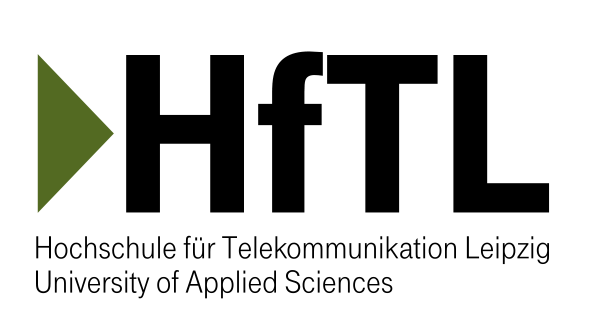
\includegraphics[width=2.5cm]{images/HfTL-Logo.png}
      \end{tabular}
      \hfill%
      \begin{tabular}[m]{c}
        Hochschule für Telekommunikation Leipzig (FH)\\
        Wirtschaftsinformatik \\
        Wissenschaftlich angeleitete Berufspraxis III\\
      \end{tabular}%
    }
  \end{center}
\end{figure}

\begin{center}
\rule{0pt}{0pt}
\vfill
\vfill
\vfill
\vfill

\begin{huge}
WAB III Projektarbeit:\\[0.75ex]
\dots\\[0.75ex]
E-Mail-Sicherheit\\[0.75ex]
\dots\\[0.75ex]
\end{huge}

\vfill
\vfill

Projektarbeit\\ von\\

\vspace*{.5cm}
Pascal Feller\\
Daniel Moy\\
Florian Schünhoff\\
Chi Cong Tran\\
\vspace{.5cm}
28. Juni 2014\\

\vfill
\vfill
\vfill
\vfill

\begin{tabular}{rl}
Referent, Betreuer:   & Prof. Dr. - Ing. Undine Pielot\\
\end{tabular}
\end{center}
\end{titlepage}



\newpage
\pagestyle{empty}


\text{ }
\vspace{11.5cm}




Hiermit versichern wir, dass wir die von uns vorgelegte Arbeit selbstständig verfasst haben, dass wir die verwendeten Quellen, Internet-Quellen und Hilfsmittel vollständig angegeben haben und dass wir die Stellen der Arbeit -- einschließlich Tabellen, Karten und Abbildungen~--, die anderen Werken oder dem Internet im Wortlaut oder dem Sinn nach entnommen sind, auf jeden Fall unter Angabe der Quelle als Entlehnung kenntlich gemacht haben.\\

Leipzig, den 28. Juni 2014\\
\medskip
\medskip

(Unterschrift)\\
\underline{~~~~~~~~~~~~~~~~~~~~~~~~~~~~~~~~~~~~~~~~}\\
Pascal Feller\\
\underline{~~~~~~~~~~~~~~~~~~~~~~~~~~~~~~~~~~~~~~~~}\\
Daniel Moy\\
\underline{~~~~~~~~~~~~~~~~~~~~~~~~~~~~~~~~~~~~~~~~}\\
Florian Schünhoff\\
\underline{~~~~~~~~~~~~~~~~~~~~~~~~~~~~~~~~~~~~~~~~}\\
Chi Cong Tran\\

\newpage


\pagestyle{empty}
%Seitenumbruch
\pagebreak

\pagenumbering{Roman}
%Inhaltsverzeichnis
\tableofcontents
\pagebreak
%Abbildungsverzeichnis
\listoffigures
\pagebreak
%falls ben�tigt auch noch ein Tabellenverzeichnis, m�sste dann die Auskommentierung aufgehoben werden
%\listoftables
%\pagebreak
%einbinden des in Akronyme.tex erstellten Abbildungsverzeichnisses
\phantomsection \addcontentsline{toc}{chapter}{Abkürzungsverzeichnis}
\renewcommand\refname{Abkürzungsverzeichnis} \chapter*{Abkürzungsverzeichnis}
\begin{acronym}[StuRa] % In die optionale eckige Klammer die längste Abkürzung schreiben (für gemeinsame Ausrichtung)
	\acro{DHE}{Diffie-Hellmann-Verfahren}
	\acro{TLS/SSL}{Transport Layer Security/Secure Socket Layer}
	\acro{PFS}{Perfect Foreward Secrecy}
\end{acronym}
\pagebreak

%�ndern der Seitennummerierung auf arabische Zahlen und Beginn bei Seite 1
\pagenumbering{arabic}\setcounter{page}{1}
%%Dies ist die Vorlage für die einzelnen Kapitel, die jeweils mit Chapter als Kapiteltitel starten
\chapter{Titel des Kapitels}

%mit \section{title} wird ein Unterkapitel der ersten Gliederungsebene überschrieben
\section{Wichtiges Unterkapitel erster Gliederungsebene}
Lorem ipsum \dots

%mit \subsection{title} wird ein Unterkapitel der zweiten Gliederungsebene überschrieben
\subsection{Wichtiges Unterkapitel der zweiten Gliederungsebene}
Lorem ipsum \dots

%Vom Grundsatz war es das für die Erstellung von Kapiteln, jetzt kommt noch ein kleines Beispiel für Fußnoten
Dies ist ein großartiges Beispiel \footnote{Wenn einem nix einfällt muss man eben Quatsch schreiben} für eine Fußnote.
%%Dies ist die Vorlage für die einzelnen Kapitel, die jeweils mit Chapter als Kapiteltitel starten
\chapter{Datensicherheit 1x1}
Unter Datensicherheit wird der Schutz von Daten in den Aspekten Verfügbarkeit, Vertraulichkeit und Integrität verstanden. \footnote(https://www.bsi.bund.de/DE/Themen/ITGrundschutz/ITGrundschutzKataloge/Inhalt/Glossar/glossar_node.html). Im Gegensatz dazu beschreibt Datenschutz den Schutz von und den vertrauensvollen Umgang mit persönlichen Daten. In der IT-Sicherheit wird zusätzlich des Aspekt der Authentizität berücksichtigt \footnote{http://www.datenschutz-berlin.de/content/technik/begriffsbestimmungen/verfuegbarkeit-integritaet-vertraulichkeit-authentizitaet}. In diesem Abschnitt werden diese Aspekte näher betrachtet, da diese für das Verstädnis der vorgestellten Techniken in den späteren Kapitel notwendig sind.

%mit \section{title} wird ein Unterkapitel der ersten Gliederungsebene überschrieben
\section{Verfügbarkeit}

Unter Verfügbarkeit wird das Vorhandensein von Infrastruktur, Software, sämtliche IT-Dienstleistungen sowie -Funktionalitäten und Daten verstanden, so dass die Anwender bei Bedarf darauf zugreifen und nutzen können. Um dies zu gewährleisten, muss verhindert werden, dass
\begin{itemize}
\item Daten verschwinden oder nicht zugreifbar sind, wenn sie gebraucht werden,
\item Programme nicht funktionsbereit sind, wenn sie aufgerufen werden sollen,
\item Hardware und sonstige notwendige Mittel nicht funktionsfähig oder gar verschwunden sind, wenn sie für die Verarbeitung benötigt wird. \footnote{http://www.datenschutz-berlin.de/content/technik/begriffsbestimmungen/verfuegbarkeit-integritaet-vertraulichkeit-authentizitaet}
\end{itemize}

\section{Integrität}
Unter der Integrität der Daten wird verstanden, dass die Daten nicht ohne Aufzufallen verändert werden können und somit vollständig übermittelt worden sind. Bei diesem Aspekt geht es demzufolge um die Unversehrtheit der Nachricht.

\section{Vertraulichkeit}

Unter Vertraulichkeit versteht man den Schutz der Nachricht vor unbefugtem Zugriff durch Dritte. Nur der gewünschte Empfänger soll in der Lage sein, den Inhalt der Nachricht zu erfahren. Dazu werden mathematische Verfahren genutzt, die in den späteren Kapiteln behandelt werden.

\section{Authentizität}

Bei der Authentizität geht es darum, nachzuweisen, dass die beteiligten Kommunikationspartner tatsächlich diejenigen sind, für die sie sich ausgeben.
%Dies ist die Vorlage für die einzelnen Kapitel, die jeweils mit Chapter als Kapiteltitel starten
\chapter{Kryptographie}
Die Kryptographie ist eine Wissenschaftslehre, die sich mit den Verfahren sowie der Anwendung von Ver- und Entschlüsselung von Informationen befasst. Dabei bedient sie sich mathematischen Hilfsmitteln, um die Daten vor Dritten unzugänglich zu machen. In diesem Kapitel werden zunächst die grundlegende Funktionsweise der Verschlüsselung untersucht, die zum Verständnis der weiteren Unterkapitel notwendig sind. Anschließend werden verschiedene Verfahren beleuchtet, die eine verschlüsselte und geschützte Kommunikation ermöglichen.
%mit \section{title} wird ein Unterkapitel der ersten Gliederungsebene überschrieben
\section{Grundlagen}


%mit \subsection{title} wird ein Unterkapitel der zweiten Gliederungsebene überschrieben
\subsection{Symmetrische Verschlüsselung}

Bei der symmetrischen Verschlüsselung wird sowohl zur Verschlüsselung und Entschlüsselung ein gemeinsamer Schlüssel verwendet. Dieser Schlüssel wird auch Shared Secret genannt. Mithilfe dieses Schlüssels und einem kryptographischen Algorithmus wird die Information des Absenders, auch als Klartext bezeichnet, verschlüsselt. Ein Algorithmus transformiert dabei einen Eingabeparameter in einen Ausgabeparameter. Im Fall eines kryptographischen Algorithmus handelt es sich um eine mathematische Vorschrift, die aus dem Klartext einen sogenannten Geheimtext berechnet. Diesen verschlüsselten Text kann der Empfänger mit dem selben Schlüssel, der zur Verschlüsselung verwendet wurde, entschlüsseln. Die folgende Abbildung zeigt das Funktionsprinzip einer symmetrischen Verschlüsselung
\footnote{Kryptographie, S. 41}
Im elektronischen Briefverkehr wirkt sich die Funktionsweise der symmetrischen Verschlüsselung nachteilig auf deren Anwendung auf. Da beide Kommunikationspartner denselben Schlüssel benötigen, muss dieser zuvor ausgehandelt und übertragen werden. Dieser Umstand stellt ein Risiko bezüglich der Vertraulichkeit dar. Jeder, der über den Schlüssel verfügt, kann auf den Inhalt der Nachricht zugreifen. Dieses Sicherheitsrisiko wird durch die asymmetrische Verschlüsselung beseitigt.

\subsection{Asymmetrische Verschlüsselung}

Wie bei der symmetrischen Verschlüsselung kommt auch bei der asymmetrischen Verschlüsselung, die auch Public-Key-Kryptography genannt wird, ein kryptographischer Algorithmus zum Einsatz. Bei letzterem Verfahren wird statt eines Schlüssels ein Schlüsselpaar verwendet. Dieser besteht aus einem öffentlichen und einem privaten Schlüssel, die mathematisch zusammenhängen. Jeder, der verschlüsselte Nachrichten empfangen möchte, verfügt über ein solches Schlüsselpaar. Der private Schlüssel wird niemals bekanntgegeben, wohingegen der öffentliche Schlüssel jedem zugänglich gemacht werden kann. Obwohl die Schlüssel zusammenhängen, kann aus der Kenntnis des öffentlichen Schlüssels nicht auf den privaten Schlüssel geschlossen werden. Möchte Alice mit diesem Verfahren eine verschlüsselte Mail an Bob versenden, so besorgt sie sich zunächst den öffentlichen Schlüssel von Bob. Damit verschlüsselt sie ihre Nachricht und schickt diese an Bob, der die Nachricht mit seinem privaten Schlüssel entschlüsseln kann. Die Abbildung verdeutlicht noch einmal die Funktionsweise der Public-Key-Verschlüsselung
\footnote{Kryptographie, S. 177}
Mit diesem Verfahren wurde das Sicherheitsrisiko der symmetrischen Verschlüsselung behoben, da der öffentliche Schlüssel zum Verschlüsseln jedem bekannt sein darf. Zur Entschlüsselung wird der dazugehörige private Schlüssel benötigt, der im Besitz des Empfängers ist und niemals veröffentlicht wird.
Ein Sicherheitsrisiko ergibt sich jedoch aus der Tatsache, dass ein Dritter die Übertragung des öffentlichen Schlüssels von Bob abfangen und sich somit als Bob ausgeben kann, indem er seinen öffentlichen Schlüssel publiziert. In diesem sogenannten Man-In-The-Middle-Szenario kann der Dritte nun alle vermeintlich an Bob verschlüsselten Nachrichten lesen, da diese mit seinem öffentlichen Schlüssel verschlüsselt worden sind.
Dies wird durch digitale Signaturen sichergestellt, deren Konzept im nächsten Kapitel näher untersucht wird.

\subsection{Digitale Signaturen}

Digitale Signaturen bieten die Möglichkeit, die menschliche Unterschrift in der digitalen Welt abzubilden. Um dies zu garantieren, müssen folgende Bedingungen eingehalten werden:
\footnote{Kryptographie S. 202}
\begin{itemize}
\item Sie darf nicht zu fälschen sein.
\item Ihre Echtzeit muss überprüfbar sein
\item Sie darf nicht unbemerkt von einem Dokument zum anderen übertragen werden können.
\item Das dazugehörende Dokument darf nicht unbemerkt verändert werden können.
\end{itemize}
Diese Voraussetzungen dienen dazu, die Authentizität sowie die Integrität des Absenders zu gewährleisten. Dazu wird das asymmetrische Verschlüsselungsverfahren genutzt. Dabei verschlüsselt der Absender seine Nachricht mit seinem privaten Schlüssel. Dieser Vorgang wird als signieren bezeichnet. Die resultierende verschlüsselte Nachricht ist die digitale Signatur. Zusammen mit der ursprünglichen Nachricht wird die Signatur zum Empfänger geschickt. Dieser kann nun die Authentizität der Nachricht überprüfen, indem er die Signatur mit dem öffentlichen Schlüssel des Absenders entschlüsselt. Stimmt die entschlüsselte Nachricht mit der originalen Nachricht überein, so kann er sicher sein, dass die Nachricht von dem Absender stammt, da nur mit dessen privatem Schlüssel die Nachricht verschlüsselt sein konnte. Zusätzlich ist damit garantiert, dass die Nachricht vollständig und ungeändert beim Absender angekommen ist.

Beim Signieren wird in der Regel aufgrund des Rechenaufwandes für lange Nachrichten nicht die gesamt Nachricht verschlüsselt, sondern ein sogenannter Hashwert der Nachricht. Hashwerte sind eine Zeichenfolge mit einer bestimmten Länge, die durch eine mathematische Einweg-Hashfunktion generiert werden. Diese Funktionen haben einen Eingabeparameter und berechnen daraus den erwähnten Hashwert. Aus der Kenntis des Hashwertes und der Funktion lässt sich der Eingabeparameter nicht ableiten. Dadurch, dass zu jedem Eingabeparameter nur ein Hashwert existiert, bleibt die Eigenschaft der Integrität erhalten.

\subsection{Zertifikate}
Bei den bisher genannten Verfahren wurde davon ausgegangen, dass der öffentliche Schlüssel wirklich dem Kommunikationspartner gehört. Die Verlässlichkeit des öffentlichen Schlüssels ist durch Szenarien wie dem Man-In-The-Middle-Angriff nicht immer garantiert. Um dies zu erreichen, werden Zertifikate benutzt.
Ein Zertifikat ist ein elektronisches Dokument, das einer Person zugeordnet werden kann. Dieses Dokument enthält neben den persönlichen und weiteren Informationen des Inhabers dessen öffentlichen Schlüssel. Außerdem enthält ein Zertifikat eine Signatur über all den genannten Angaben. Das Signieren wird dabei meist von einer vertrauenswürdigen Instanz durchgeführt, die auch \ac{CA} oder Zertifizierungsstelle genannt wird.
Möchte Alice Bob nun eine verschlüsselte Nachricht schicken, so besorgt sich Alice zunächst Bobs Zertifikat, auf dem sich dessen öffentlicher Schlüssel befindet. Um zu prüfen, ob dieser Schlüssel tatsächlich zu Bob gehört, verifiziert sie nun sein Zertifikat, indem sie die Signatur mit dem öffentlichen Schlüssel der \ac{CA} entschlüsselt. Stimmen beide Schlüssel überein, kann sie davon ausgehen, dass dieser Schlüssel tatsächlich Bob gehört.
Das Sicherheitsrisiko bezüglich der Verlässlichkeit des öffentlichen Schlüssels der Zertifizierungsstelle wird so gelöst, indem ein Zertifikat über den öffentlichen Schlüssel erstellt wird, das von der CA selbst signiert wurde. Dieses Zertifikat wird als self-signed bezeichnet.

\section{Web of Trust}
Das Web of Trust ist ein Vertrauensmodell, bei dem sich die Nutzer gegenseitig vertrauen und somit ein netzartiges Modell entstehen lässt. Die Grundidee ist dabei, dass die Nutzer die öffentlichen Schlüssel voneinander signieren. An einem Beispiel lässt sich das Grundprinzip dieses Modells verdeutlichen \footnote{Angewandte Kryptographie, S. 120}: Carol möchte Bob eine vertrauliche Nachricht schicken. Dazu besorgt er sich Bobs öffentlichen Schlüssel. Zuvor hatte Alice den öffentlichen Schlüssel von Bob signiert. Da Carol Alice vertraut, beschafft sie sich die Signatur von Alice über den öffentlichen Schlüssel von Bob und entschlüsselt diesen mit Alices öffentlichem Schlüssel. Stimmen die Schlüssel überein, so kann Carol den öffentlichen Schlüssel von Bob vertrauen, weil dieser von Alice signiert wurde, der Carol vertraut. Die folgende Abbildung veranschaulicht das Funktionsprinzip:
\footnote{S. 121, Angewandte Kryptographie}.
Bei diesem Modell wird zwischen zwei Arten des Vertrauens unterschieden. Zum einen vertraut man in einen Schlüssel, indem dieser Schlüssel durch jemand anderes, den man vertraut, signiert worden ist. Zum anderen gibt es das Vertrauen in eine Person. Diese beiden Arten sind nicht voneinander abhängig.
%Dies ist die Vorlage für die einzelnen Kapitel, die jeweils mit Chapter als Kapiteltitel starten
\chapter{Schlüsselaustausch}

%mit \section{title} wird ein Unterkapitel der ersten Gliederungsebene überschrieben
\section{Perfect Forward Secrecy - PFS}
%Problem
Beim klassischen Schlüsselaustausch werden die Sitzungsschlüssel durch den Public Key innerhalb des Server-Zertifikat übertragen.\footnote{Golem} Dies geschieht mittels RSA-Verfahren. Verschlüsselte Kommunikation ist jedoch nur solang die Schlüssel geheim bleiben sicher. Die Gefahr beim klassischen RSA-Public-Key-Verfahren ist dass vergangene Kommunikation nachträglich zu jedem Zeitpunkt entschlüsselt werden kann, sobald Angreifer in Besitz des Private Keys sind. 

%Idee
Sinnvoller ist es die Sitzungsschlüssel %REFERENZ Erklären was Sitzungsschlüssel sind
zum Einen nicht mehr zu übertragen und zum Anderen unabhängig voneinander ständig neu zu generieren und bei Terminierung zu löschen. 
Realisiert wird dies durch die Protokoll-Eigenschaft Forward Secrecy, die im Kryptographischen Fachjargon auch \ac{PFS}\footnote{golem} genannt wird.

%Umsetzung
Das \ac{DHE} ermöglicht die Aushandlung eines Sitzungsschlüssels bei dem die Kommunikationsparter verschiedene Nachrichten senden und sich auf einen Sitzungsschlüssel einigen können, ohne diesen je übertragen zu haben. Dieser Schlüssel ist auch nur für die aktuelle Verbindung gültig und wird anschließend gelöscht. Der Public-Key des Servers wird weiterhin übertragen, jedoch nur um den Schlüsselaustausch zu signieren. Die Verschlüsselungsverfahren \ac{TLS/SSL} und IPsec beherrschen bereits \ac{PFS}.

%Vorteile
Aufgezeichnete verschlüsselte Daten können somit bei Besitz des privaten Schlüssels nicht entschlüsselt werden. Zudem wird einfaches Belauschen einer aktiven Verbindung deutlich erschwert, denn es müsste die gesamte Kommunikation mit einem gezieltem Man-in-the-Middle Angriff manipuliert werden. Für diese Problematik gibt es wiederum moderne Ansätze wie DANE, die in Kombination mit PFS aktuell bei der Verschlüsselung von Verbindungen höchsten Sicherheitsansprüchen entsprechen, indem zusätzlich die Authentizät der Kommunikation gewährleistet wird. %REFERENZ MitM erklären 

%Nachteile
Nachteile gibt es lediglich bei der Verwendung des bereits überholten, und seit Jahren als geknackt bekannte DHE-Verfahren, denn dabei verzögert sich zusätzlich der Verbindungaufbau. Die Moduluslänge der Schlüssel ist Minimum 1024 Bit, und längere Schlüssel mit 2048 oder 4096 Bit sind debi nicht sicher. Der moderne Nachfolger mit elliptischen Kurven (ECDHE) gilt aktuell als sicher und benötigt dabei weniger als 1024 Bit und verzögert den Verbindungsaufbau nur unweigerlich. 

%Grenzen
Obwohl es Forward Secrecy bereits seit 1999 im TLS Standard 1.0 \footnote{golem} vorgesehen ist und smoit essenzieller Bestandteil von Verschlüsselung ist, hat sich PFS nocht nicht als Standard durchgesetzt.\footnote{https://www.trustworthyinternet.org/ssl-pulse/} Dies liegt zum einen an den Webservern. Mit einem Apache Webserver ist nur eine Moduluslänge von 1024 Bit vorgesehen. Beim Einsatz von DHE würden Provider damit ihre Server also unsicher betreiben. Zum Anderen sind es auf Client-Seite die Browser die noch nicht mitspielen. Der InternetExplorer verschlüsselt nur nach DSS, wobei der de-facto Standard für verschlüsselung RSA ist. Opera unterstützt lediglich das überholte DHE-Verfahren und Safari priorisiert Forward Secrecy niedrig und bevorzugt bei gegebener Option sogar die unverschlüsselte Kommunikation. Lediglich Firefox und Chrome unterstützen PFS in volle Umfang. 

%Browser prüfen und mit eigenen Quellen versehen
%Dies ist die Vorlage für die einzelnen Kapitel, die jeweils mit Chapter als Kapiteltitel starten
\chapter{Transportwegverschlüsselung}
Das \ac{SSL}-Protokoll wurde zunächst durch die Firma Netscape entwickelt, um die Kommunikation über \ac{HTTP}-Verbindungen abzusichern.\footcite[S. 796]{Eckert2013} \ac{SSL} kann auf der Sitzungs- und Präsentationsschicht des \ac{OSI}-Referenzmodells angesiedelt werden und setzt meist auf dem \ac{TCP} auf. Es hat die Aufgabe den darüber liegenden Schichten die Möglichkeit für eine authentifizierte, integritätsgeschützte und verschlüsselte Kommunikation zu geben.\footcite[Vgl.][S. 799 ff.]{Eckert2013}
Die Version \ac{SSL} 3.0 hat sich mittlerweile als de facto Standard im Internet durchgesetzt und wird von allen gängigen Browsern unterstützt.

Das \ac{TLS}-Protokoll kann als Weiterentwicklung von \ac{SSL} 3.0 angesehen werden und liegt aktuell in der Version 1.2 vor.
Da beide Protokolle in ihren Kernkonzepten übereinstimmen werden sie häufig synonym verwandt. Da \ac{TLS} jedoch eine Weiterentwicklung von \ac{SSL} ist, werden dort einige Erweiterungen eingeführt sowie unsichere Verfahren zur Berechnung von \ac{MAC}-Werten durch neuere Varianten ersetzt.\\
\begin{wrapfigure}{r}{0.5\textwidth}
	\begin{center}
		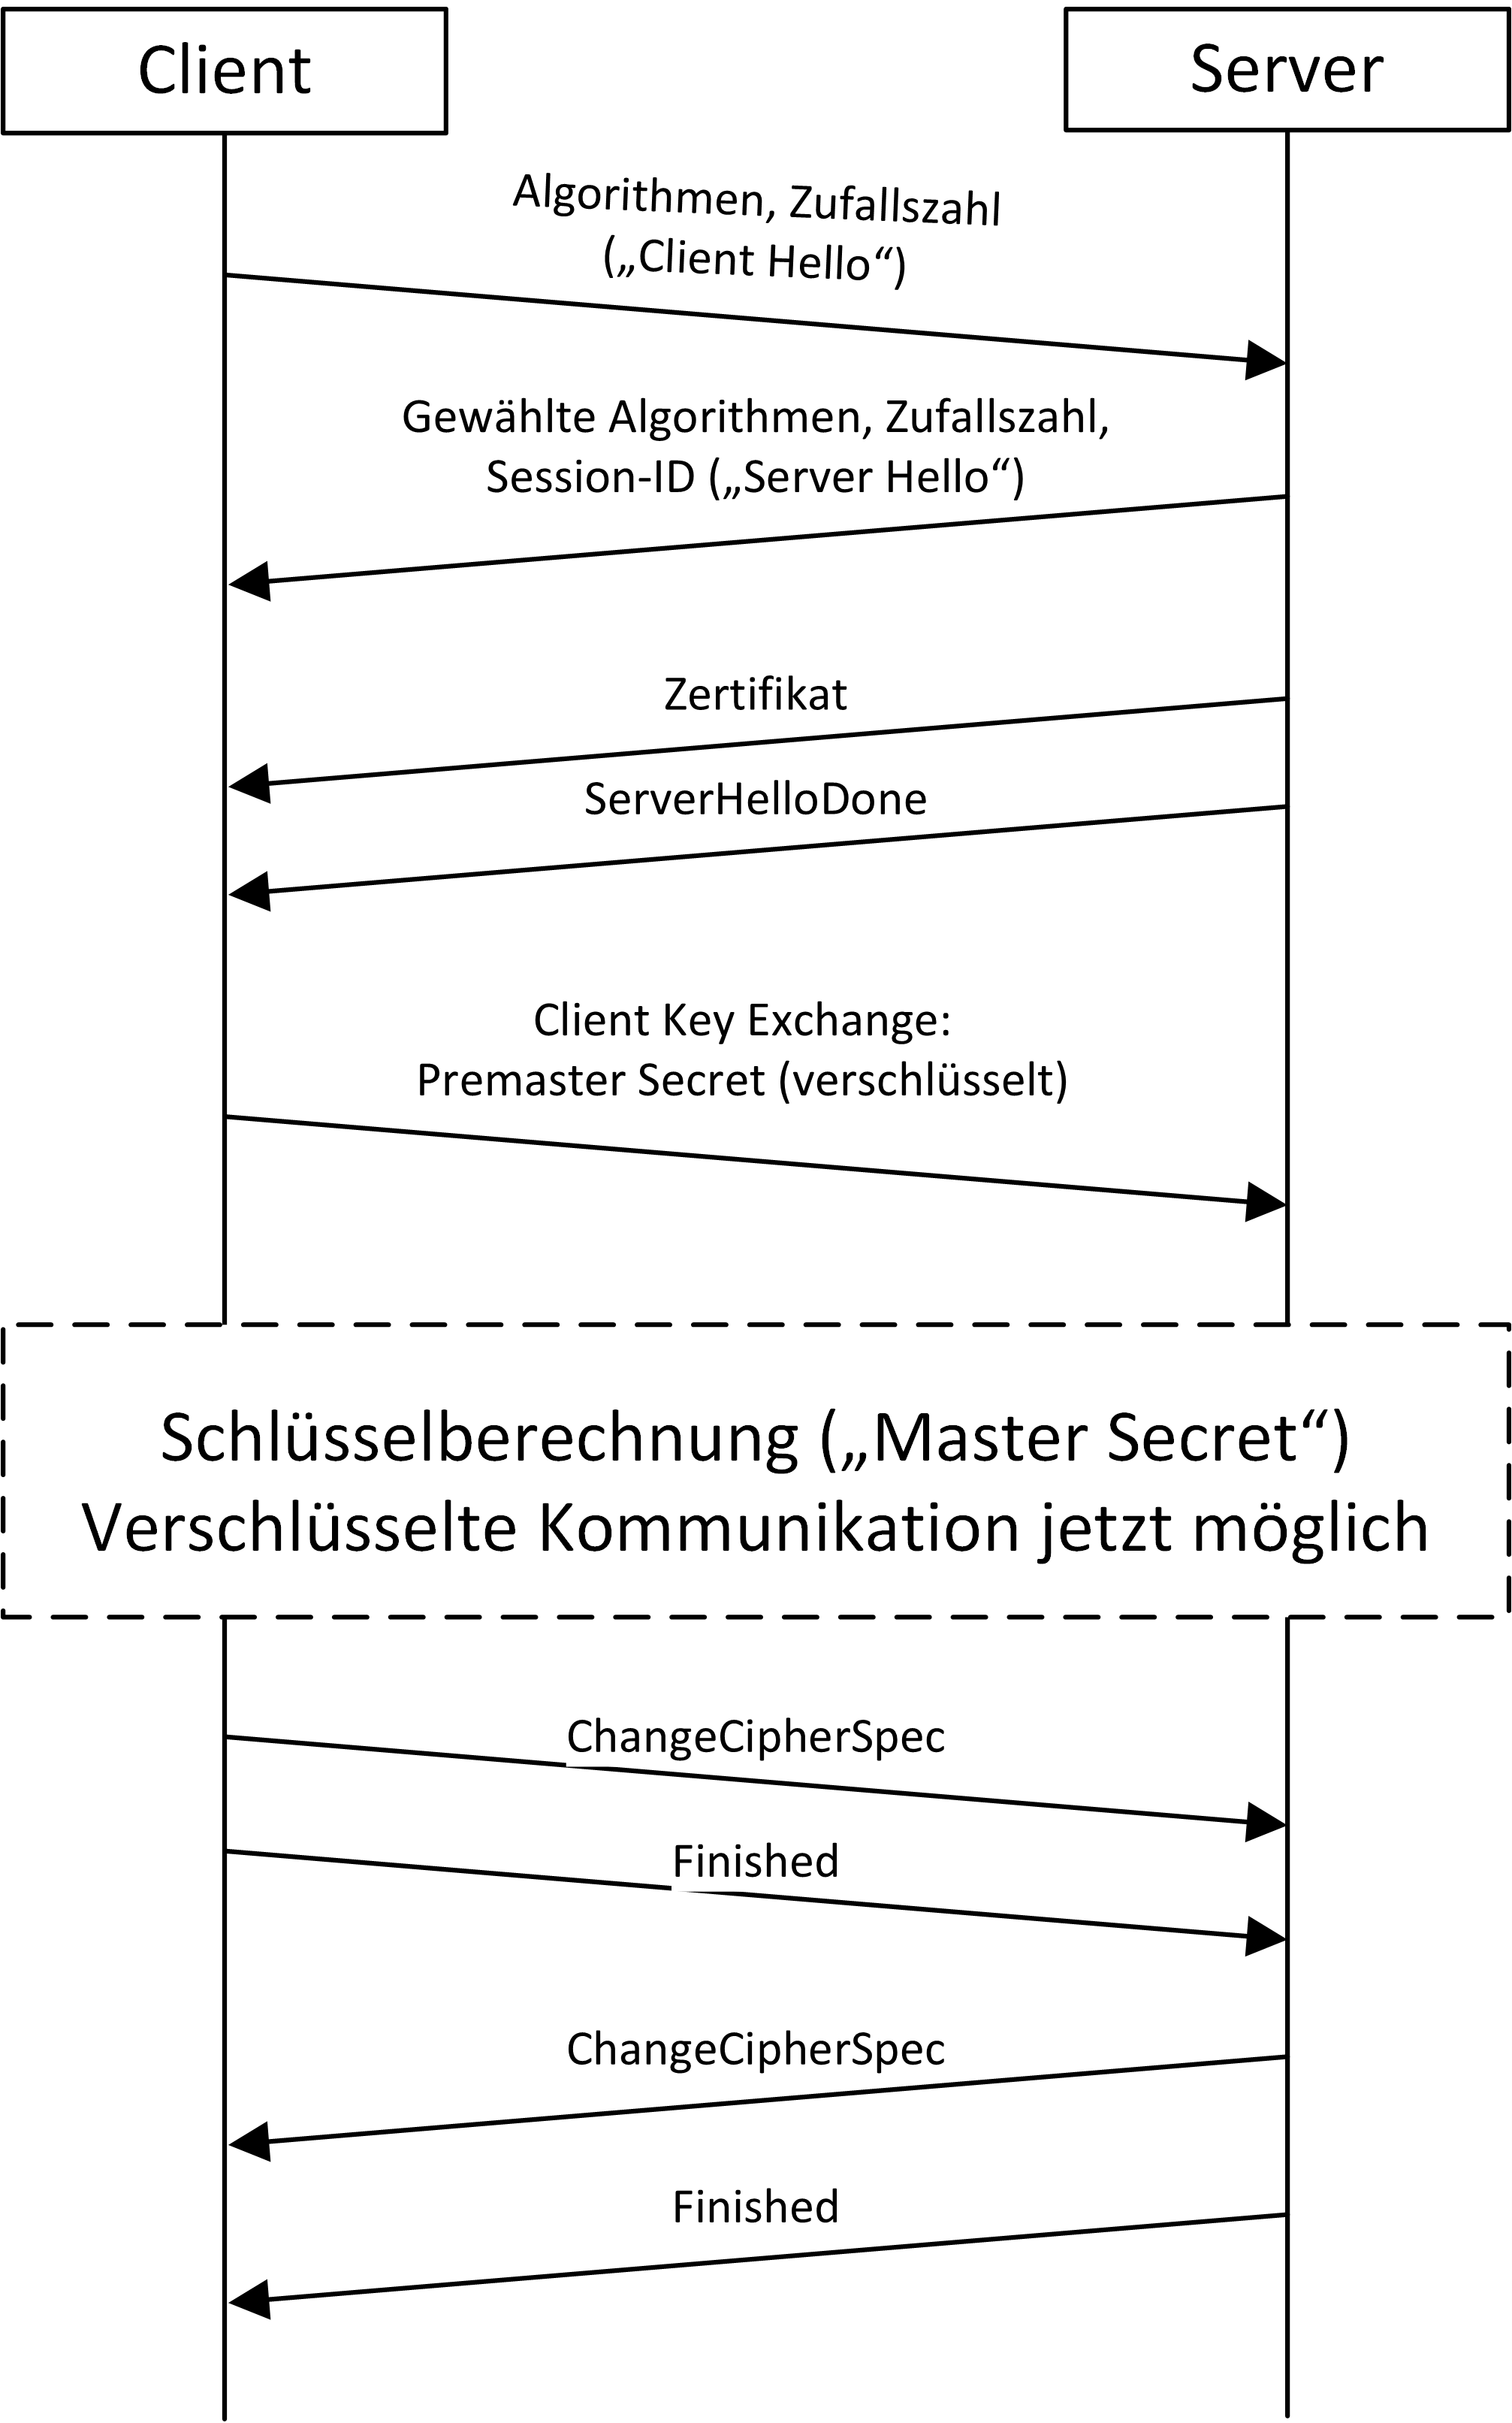
\includegraphics[width=0.4\textwidth]{images/MSC_Transport.png}
	\end{center}
	\caption{Handshake-Protokoll mit RSA}
	\footcite[In Anlehnung an][S. 170]{Sorge2013}
	\label{MSC_Transport}
\end{wrapfigure}

Beide Protokolle bestehen aus mehreren Schichten bzw. Unterprotokollen wobei das Record- und das Handshakeprotokoll von besonderer Bedeutung sind. 
Das Record-Protokoll ist für die Fragmentierung, Authentifizierung mittels \ac{MAC} und Verschlüsselung der zu übertragenden Daten zuständig. 
Mittels des Handshakeprotokolls werden Sitzungen zwischen den Kommunikationspartnern hergestellt. 
Dies bedeutet, dass die Kommunikationspartner durch den Austausch von Zertifikaten authentifiziert werden können und alle Informationen, die zur Berechnung des Shared Secret für die symmetrische Verschlüsselung der Daten benötigt werden, ausgetauscht werden. 
Die folgende Abbildung verdeutlicht den schematischen Ablauf eines solchen Sitzungsaufbaus unter Verwendung von \ac{RSA} für den Schlüsselaustausch.

Durch die flexible Gestaltung des Handshake-Protokolls wird gleichzeitig auch die Komplexität von \ac{TLS/SSL} stark erhöht. 
Dies hat zur Folge, dass durch die hohe Komplexität nicht mit Sicherheit alle Schwachstellen beim Design des Protokolls entfernt werden konnten. 
Außerdem ist zu bedenken, dass \ac{TLS/SSL} aufgrund seiner weiten Verbreitung ein lohnendes Ziel für Angriffe ist. Die Sicherheit des Protokolls hängt dabei stark von den genutzten kryptologischen Methoden ab. 
Außerdem ist zu beachten, dass es sich, aufgrund der Ansiedlung des Protokolls unterhalb der Anwendungsschicht, nur um eine Verschlüsselung der transportierten Nutzdaten auf dem Transportweg handelt. 
Die Daten werden am Kommunikationsendpunkt entschlüsselt und anschließend an die entsprechende Anwendung weitergereicht.

Auch die Authentifizierung der Kommunikationspartner mittels Zertifikaten weißt dieselben Schwachstellen durch die Vertrauensbeziehung zu bekannten \ac{CA}s, die unzureichend gesichert sind, auf.  

An dieser Stelle kann dann mal probiert werden ob Flaschenhals jetzt korrekt getrennt wird in dem ganz oft Flaschenhals geschrieben wird: Flaschenhals Flaschenhals Flaschenhals Flaschenhals Flaschenhals Flaschenhals Flaschenhals Flaschenhals Flaschenhals Flaschenhals
%Wenn automatisch erzeugtes Literaturverzeichnis verwendet wird, wird es hier eingef�gt
%\printbibliography

\end{document}